\documentclass[twoside]{article}
\usepackage[utf8]{inputenc}
\usepackage{lipsum} % Package to generate dummy text throughout this template
\usepackage[sc]{mathpazo} % Use the Palatino font
\linespread{1.05} % Line spacing - Palatino needs more space between lines
\usepackage{microtype} % Slightly tweak font spacing for aesthetics
\usepackage[hmarginratio=1:1,top=32mm,columnsep=20pt]{geometry} % Document margins
\usepackage{multicol} % Used for the two-column layout of the document
\usepackage[hang, small,labelfont=bf,up,textfont=it,up]{caption} % Custom captions under/above floats in tables or figures
\usepackage{booktabs} % Horizontal rules in tables
\usepackage{float} % Required for tables and figures in the multi-column environment - they need to be placed in specific locations with the [H] (e.g. \begin{table}[H])
\usepackage{hyperref} % For hyperlinks in the PDF
\usepackage{lettrine} % The lettrine is the first enlarged letter at the beginning of the text
\usepackage{paralist} % Used for the compactitem environment which makes bullet points with less space between them
\usepackage{abstract} % Allows abstract customization
\usepackage{graphicx}
\renewcommand{\abstractnamefont}{\normalfont\bfseries} % Set the "Abstract" text to bold
\renewcommand{\abstracttextfont}{\normalfont\small\itshape} % Set the abstract itself to small italic text
\usepackage{titlesec} % Allows customization of titles
\renewcommand\thesection{\Roman{section}} % Roman numerals for the sections
\renewcommand\thesubsection{\Roman{subsection}} % Roman numerals for subsections
\titleformat{\section}[block]{\large\scshape\centering}{\thesection.}{1em}{} % Change the look of the section titles
\titleformat{\subsection}[block]{\large}{\thesubsection.}{1em}{} % Change the look of the section titles
\usepackage{fancyhdr} % Headers and footers
\pagestyle{fancy} % All pages have headers and footers
\fancyhead{} % Blank out the default header
\fancyfoot{} % Blank out the default footer
\fancyhead[C]{Cellular automata seminar, final assignment $\bullet$ June 2014 $\bullet$ MCIC IIMAS } % Custom header text
\fancyfoot[RO,LE]{\thepage} % Custom footer text
%----------------------------------------------------------------------------------------
%	TITLE SECTION
%----------------------------------------------------------------------------------------

\title{\vspace{-15mm}\fontsize{24pt}{10pt}\selectfont\textbf{Cellular automata simulation for portfolio execution strategies}} % Article title

\author{
\large Fabián Romero \\ % 
\normalsize University of Mexico (UNAM) \\ % Your institution
\normalsize \href{mailto:fromeroj@gmail.com}{fromeroj@gmail.com} % Your email address
\vspace{-5mm}
}
\date{}

%----------------------------------------------------------------------------------------

\begin{document}

\maketitle % Insert title

\thispagestyle{fancy} % All pages have headers and footers

%----------------------------------------------------------------------------------------
%	ABSTRACT
%----------------------------------------------------------------------------------------

\begin{abstract}

\noindent 
Market impact is defined as the change of the price of a stock produced for a trade action. Defined by Kyle \cite{Kyle1985} whom also noticed it is directly related to the size of the trade. \\
Should a trader require sell or buy a large amount of stock as close as possible to current market's price. Has to consider the effect and timing for her actions.
If she trades too slow, prices may move away because the dynamic nature of the market (market's risk). If she trades too fast, it will produce a larger impact. Minimizing both, the risk, and the impact created by this transaction is the goal of an execution strategy.\\
For this work we introduce and measure an execution strategy. 
We assume a simplistic stock market where only two criteria are set for acceptable simulation of market's behaviour.
Black–Scholes ({\bf BS}) \cite{black1973poa} model for the market itself.
And Kyle's impact equations for market's impact. We choose to use cellular automata because they can accurately model market's complex dynamics with simplicity and computational efficiency.
\end{abstract}

%----------------------------------------------------------------------------------------
%	ARTICLE CONTENTS
%----------------------------------------------------------------------------------------

\begin{multicols}{2} % Two-column layout throughout the main article text

\section{Introduction}

\subsection{Human disadvantage in trading}

\lettrine[nindent=0em,lines=3]{A}s nobel laureate Professor Vernon L. Smith explains \cite{smith2009}, humans have emotional bias such as personal preferences, herd behaviour, panic, stress induced performance degradation, etc. Which hinders sound decision making. Not to mention to be outright incapable to react in the millisecond time scale.\\

However, computers can trade reactively, accurately and unemotionally in that environment. Unsurprisingly they took the lead on the trading floor. High-frequency trading (HFT) is the use of computer algorithms to rapidly exchange securities. And, fast becoming the norm for trading.

Even traditional traders with ``regular'' assets and strategies, have to adapt to this reality, as Michel Lewis explains on its best-seller \cite{lewis2014},  “You could see that when you were trading a stock, the market knew what you were going to do, and it was going to move against you.”. To conclude ``the market is rigged''.

Meanwhile it is true that today algorithmic traders have a large advantage indeed, it is also true that is up to the traders to implement new technology and benefit as well. And to be able to perform without losing to algorithmic traders.

\subsection{Execution algorithms}

There are many execution algorithms which are used, we will describe some of them to illustrate their variety:

\begin{itemize}
\item Impact-driven algorithms\\
They aim to minimise market impact by slicing a big trading order into smaller child
orders.\\
Examples: time-weighted average price, volume-weighted average price and
percent of volume
\item Cost-driven algorithms\\
They try to reduce the efect of overall transaction costs such as market impact and
market risk.\\
Examples: implementation shortfall and target close
\item Opportunistic algorithms\\
They seek to take advantage whenever market conditions (price, liquidity, volatility
or another factor) are favorable\\
Examples: price inline and liquidity-driven
\end{itemize}

Of course any combination of them will be a valid strategy, depending of the specific goals of a trade. In this work we focus on impact driven algorithms because we have little information on the market.

\subsection{Market models with cellular automata}

In order to choose a model which would fit the requirements of our work, we looked upon several works which provide interesting ideas and concepts.\\

M. Bartolozzi \cite{PhysRevE.69.046112} created a stochastic cellular automata, where a direct percolation method induced a hierarchy of clusters, capable of simulate ``herd behaviour'' on the stock market, it also considers three states, corresponding to ``sell'', ``buy'' and ``hold''.\\

G. Qiu. \cite{qiu2007understanding} introduced a model, which can be used on a percolation graph or a two dimensional cellular automata, creating agents with distinctive behaviour which will model ``real'' behaviours of people, and looking for market characteristics to emerge, specifically, non-Gaussian distribution of return, short-term auto correlation of return and long-term auto correlation of volatility.\\
 
Yuying Gao \cite{yuying2005}, on his doctoral thesis creates a full analytic framework and compares it with other simulation methods, modelling the behaviour of the market from the standard {\bf BS}, diffusion, spread analysis, and applying distinct methods to discretise the model. Various ideas on his work are quite enlightening, unfortunately, we could not find any code or executable version of his work.\\

\section{Our model}


\subsection{Considerations}

The most accepted model for market behaviour is Black-Stockes equation, which assume Brownian movement for the price. This model is a diffusion process, and has its roots in econophysics.\\

\begin{equation}
\label{eq:bs}
  \frac{\partial V}{\partial t}+\frac{1}{2}\sigma^2S^2\frac{\partial^2 V}{\partial S^2}+rS\frac{\partial V}{\partial S} - rV =0 
\end{equation}

Black-Scholes {\bf BS} (\ref{eq:bs}). equation, where:\\
$\sigma$ volatility,\\
$V$ price of the derivative,\\ 
$t$ time,\\ 
$r$ money's cost,\\
$S$ stock's price.\\



{\bf BS} equation explains the overall behaviour of the market as a whole. But it can be deduced from the perspective of a single actor trading a single stock portfolio. Field's medallist Terrence Tao \cite{tao2008} published an article where he derives the {\bf BS} equation, from the point of view of a single agent in a discrete time model. Quote from the article ``I only considered a discrete model rather than a continuous one, which makes the mathematics much more elementary. (...) The emphasis here will be on the simplest models rather than the most realistic models, in order to emphasise the beautifully simple basic idea behind the derivation of this formula.''. \\

His formula is:
\begin{equation}
\label{eq:tt}
log S_{t+dt}=log S_t + \mu dt + \sigma \epsilon_t(dt)^{\frac{1}{2}}
\end{equation}
Where $\mu$ measures the expected relative increase in value per unit time.\\

Consider that most of the models of cellular automata follow one of the following choices. Or they try to describe an agent behaviour and then hope for the resulting model to behave as {\bf BS}, and then proving this is the case. Or they discretise {\bf BS} and whatever the resulting formula is, it will be applied as the behaviour of the agent. In the first case, proving the behaviour with mathematical rigour can be a complex task. In the second case, arguing the rationale as an individual agent can be lacking, and any change from there will need to be back traced to the equations. With this formulation, we have a simple, discrete and elegant model for the behaviour of an agent which by construction will lead to an overall {\bf BS} behaviour of the market.\\

\subsubsection{Description}

Our model, will be based on Yuying Gao's, but with several changes that will help to introduce execution strategies, and inside Terrence Tao's framework.\\

It will be a one dimensional cellular automata, having a fuzzy state in $[0,1]$ where $[0,\frac{3}{8}]$ is ``sell'',$(\frac{3}{8},\frac{5}{8})$ is ``hold'',  $[\frac{5}{8},1]$ is ``buy''.

We implemented a variation of rule 90. We choose rule 90 after Gao's work where is shown to yield a Brownian movement as desired given random initial conditions.\\

The variation is a Fuzzy logic interpretation.
The Boolean form of rule 90 is: $p \oplus r $\\

We want to use a continuous model. So, we choose a fuzzy logic interpretation of this formula. In \cite{Hernandez2011} deduces. the operation which is the least sensitive on average has the form $f_{\oplus}(a,b)=a+b-2ab$.\\

hence rule 90 is: $ p + r - 2pr$\\

The default value of a cell is $\frac{1}{2}$.

We chose this continuous function for evaluation, then the diffusion will be smooth.\\

We define $\delta_{sell}(t,i)$ as the numbers of ``sell'' cells on time $t+i$ minus the number of ``sell'' cells on time $t$. The same for $\delta_{buy}(t,i)$ and $\delta_{hold}(t,i)$. Then define $$\Delta(t,i) = \frac{\delta_{sell}(t,i)-\delta_{buy}(t,i)}{\#cells}$$

On Kyle's original work, impact is linear. We will use that definition. And then we will impact price with the formula $$P(t+1)=P(t)*\Delta(t,1)*c$$ where $c$ is a constant. We did typically use $c=2$.



\section{Results}

\subsection{Diffusion}
Being {\bf BS} a diffusion equation we were trying to replicate Gao's findings.\\
His model is also continuous, but he shows diffusion only as a probability, where we used the fuzzy model, the following image shows side by side the results.

\begin{center}
  \includegraphics{sbs.png}\\
  Left Gao's, right ours (50 ticks).
\end{center}


\subsection{Brownian movement}
We were also trying to see how a typical stock market Brownian movement will look under this model

\begin{center}
  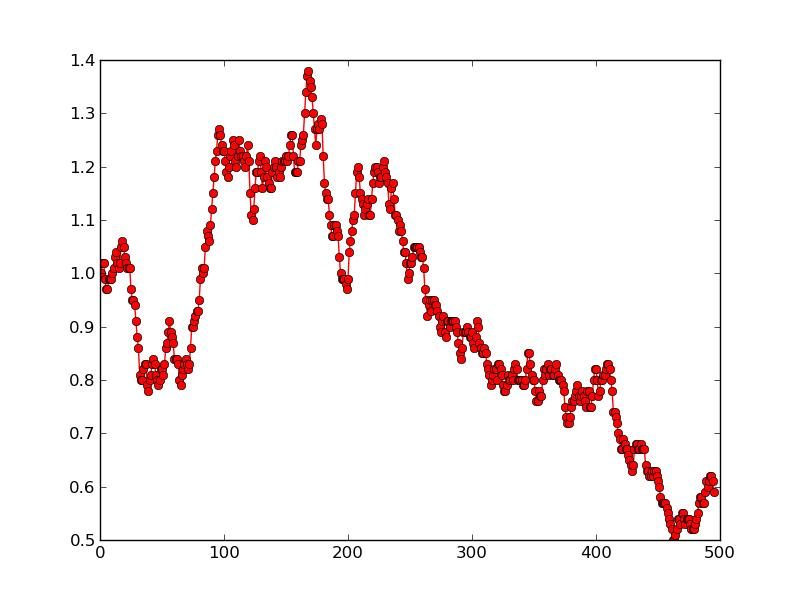
\includegraphics[width=200px]{grafica4.jpg}\\
\end{center}

This images represents price movement in a 5,000 cells {\bf AC}, running 5,000 ticks, sampling every 10 steps and using wolfram's rule 30. \\

To simulate the model proposed, the typical size of the automata we used is 10,000 cells.
We actually used $$P(t+50)=P(t)*\Delta(t,50)*2$$ and even $$P(t+100)=P(t)*\Delta(t,100)*2$$
the larger gaps allow the market to reflect the true movement before calculating price, otherwise, the price functions is attenuated, still reflecting the parameters, but doesn't has many ``quick turns'' we would expect from a Brownian movement.

So, the typical result was about 10,000 cells and 10,000 ticks, we have a custom made implementation for this work and we were able of creating this test in about $15ms$ and most notably we did this without compromising parallelism, so, we can test much bigger sets in commodity hardware.

Diffusion property is very similar to .\\

For modelling a portfolio execution, we calculate the volume, in our case we used $10\%$ of total volume. So, if the execution strategy say ``buy 1\%'' at time $t$, we take $1\%$ of the cells randomly, and set them to $1$, as the induced data structure we used is immutable, we can start with the square grid with the complete execution already in place, and run then the simulation.
 
We make a simple impact algorithm by slicing the $10\%$ impact in 1, 10, 50, and 100 slices. running this 100 times and getting the average price change.\\

The results were:

\begin{tabular}{l*{6}{c}r}
Slices & Price change\\
\hline
1   & 19.043\% \\
10  & 16.964\% \\
50  & 15.865\% \\
100 & 14.732\% \\
\end{tabular}

Which are within 5\% from Almgren's \cite{Almgren2005} theoretical results.
We did have to play with the constant for the case of full execution, we used the same constant for all other cases.


\section{Conclusions and future work}

Cellular automata can be use to simulate a stock market, and not just the market, but many of the emergent characteristics or systems which make use of a market, in the case of the current work, execution strategies are an important topic in algorithmic trading, and we think we can improve this work in order of being able of implement more complex strategies realistically. Even being able of ``dissect'' a market, so all trades in a day will be considered, except for a portfolio, and then try to understand the impact of this portfolio execution, and verify its optimal.

Whit respect to use another topology, we could use a percolation. However, we want to try to go as far as possible without compromising parallelism, and we found no substantial advantage on simulating such thing as herd behaviour, which apparently emerges from the automata itself.

%----------------------------------------------------------------------------------------
%	REFERENCE LIST
%----------------------------------------------------------------------------------------

\bibliography{bibliography} % Use the bibliography.bib file for the bibliography
\bibliographystyle{plainnat} % Use the plainnat style of referencing

%----------------------------------------------------------------------------------------
\end{multicols}
\end{document}
